\documentclass[10pt]{beamer}

\usetheme{metropolis}
\definecolor{WiLabRed}{RGB}{197,18,48}
\setbeamercolor{frametitle}{fg=white,bg=WiLabRed}
\setbeamercolor{progress bar}{fg=WiLabRed!90}
\setbeamercolor{title separator}{fg=WiLabRed!90}
\setbeamercolor{progress bar in section page}{fg=WiLabRed!90}
\setbeamercolor{background canvas}{bg=white}
\setbeamercolor{alerted text}{fg=WiLabRed!90}

\usepackage{appendixnumberbeamer}

\usepackage{booktabs}
\usepackage[scale=2]{ccicons}

\usepackage{pgfplots}
\usepgfplotslibrary{dateplot}

\usepackage{xspace}
\newcommand{\themename}{\textbf{\textsc{metropolis}}\xspace}

\usepackage{marvosym}
%\usepackage{subfig}
\usepackage{graphicx}\graphicspath{{images/}}
\usepackage{subcaption}
\usepackage[framed]{mcode}
\usepackage{listings}

\title{Lecture 22: Correlator Receiver Realization}
\subtitle{\textit{Software Defined Radio for Engineers} (Collins~\textit{et al.}), \textsection{4.7.2}}
\date{}
\author{\textbf{Alexander M. Wyglinski, Ph.D.}}
\institute{ \vspace*{1in}\hfill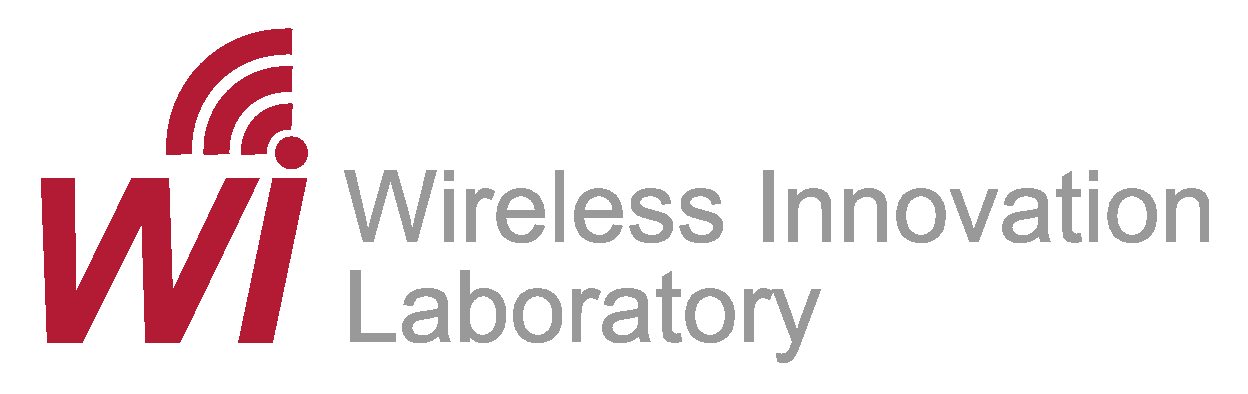
\includegraphics[height=1.125cm]{wilab_logo-A70916.eps} \qquad 
\includegraphics[height=1.125cm]{WPI_Inst_Prim_FulClr.eps}}
% \titlegraphic{\hfill\includegraphics[height=1.5cm]{logo.pdf}}

% Foot for all slides
\setbeamertemplate{frame footer}{\tiny \copyright~2018 by Alexander Wyglinski. This work is licensed under the Creative Commons Attribution-ShareAlike 4.0 International License. To view a copy of this license, visit http://creativecommons.org/licenses/by-sa/4.0/.}

\begin{document}

%\captionsetup[subfigure]{labelformat=empty}

%%%%%%%%%%%%%%%%%%%%%%%%%%%%%%%%%%%%%%%%%%%%%%%%%%%%%%%%%%

\maketitle




%%%%%%%%%%%%%%%%%%%%%%%%%%%%%%%%%%%%%%%%%%%%%%%%%%%%%%%%%%

\frame
{
  \frametitle{AWGN Vector Channel}

  \begin{itemize}
    \item Refer to Lecture 11 regarding optimal detection
    \begin{itemize}
        \item The optimal detector is equal to:
        \begin{equation}
            \max\limits_{\mathbf{s}_i}{p(\mathbf{\rho}|\mathbf{s}_i)P(\mathbf{s}_i)},~\mathsf{for}~i=1,2,\ldots,M
        \end{equation}
        \item When $P(\mathbf{s}_i)=\frac{1}{M}$ for all $i$, we get:
        \begin{equation}
            \max\limits_{\mathbf{s}_i}{p(\mathbf{\rho}|\mathbf{s}_i)},~\mathsf{for}~i=1,2,\ldots,M
        \end{equation}
    \end{itemize}
    \item The received signal is equal to:
    \begin{equation}
        \mathbf{r}=\mathbf{s}_i+\mathbf{n}
    \end{equation}
    and if we isolate for $\mathbf{n}$, we get:
    \begin{equation}
        \mathbf{n}=\mathbf{r}-\mathbf{s}_i
    \end{equation}
  \end{itemize}

}

\frame
{
  \frametitle{Manipulating the Gaussian Noise PDF}

    \begin{itemize}
        \item Recall that the joint probability density function of the noise vector $\mathbf{N}$ is equal to:
        \begin{equation}
            p(\mathbf{n})=p(n_1,n_2,\ldots,n_N)=\frac{1}{(2\pi\sigma^2)^{N/2}}{e^{-||\mathbf{n}||^2/2\sigma^2}}
        \end{equation}
        \item We can easily show that the conditional probability density function of $\mathbf{\rho}$ given $\mathbf{s}_i$ is equal to:
        \begin{equation}
        \begin{split}
            p(\mathbf{\rho}|\mathbf{s}_i)&=p(\mathbf{\rho}-\mathbf{s}_i)=p(\mathbf{n})\\
            &=\frac{1}{(2\pi\sigma^2)^{N/2}}{e^{-||\mathbf{\rho}-\mathbf{s}_i||^2/2\sigma^2}}
        \end{split}
        \end{equation}
        \begin{itemize}
            \item Vector $\mathbf{s}_i$ is a fixed quantity that is known
            \item Vector $\mathbf{\rho}$ is simply the addition of $\mathbf{s}_i$ with a Gaussian noise vector $\mathbf{n}$
        \end{itemize}
    \end{itemize}

}

\frame
{
  \frametitle{Uncorrelated Gaussian Noise Vector}

    \begin{itemize}
        \item Suppose we consider a single element of these vectors, say the $k^{\mathsf{th}}$ element:
        \begin{equation}
            p({\rho}_k|{s}_{ik})=\frac{1}{\sqrt{2\pi\sigma^2}}{e^{-({\rho}_k-{s}_{ik})^2/2\sigma^2}}
        \end{equation}
        \item Since we assume that the AWGN vector elements are uncorrelated (i.e., independent), we have:
        \begin{equation}
            p(\mathbf{\rho}|\mathbf{s}_i)=\prod\limits_{k=1}^{N}p({\rho}_k|{s}_{ik}),~\mathsf{for}~i=1,2,\ldots,M
        \end{equation}
        \item Consequently, this product of elemental probability density functions will yield:
        \begin{equation}
            p(\mathbf{\rho}|\mathbf{s}_i)=\frac{1}{(2\pi\sigma^2)^{N/2}}{e^{-||\mathbf{\rho}-\mathbf{s}_i||^2/2\sigma^2}}
        \end{equation}
    \end{itemize}

}

\frame
{
  \frametitle{Maximum Likelihood Detector}

  \begin{itemize}
    \item For the maximum likelihood detector case, we want $\max\limits_{\mathbf{s}_i}{p(\mathbf{\rho}|\mathbf{s}_i)}$
    \item Suppose we take the expression for $p(\mathbf{\rho}|\mathbf{s}_i)$, apply it to the ML detector, and take the natural logarithm, yielding:
    \begin{equation}
        \ln(p(\mathbf{\rho}|\mathbf{s}_i))=\frac{N}{2}\ln\left(\frac{1}{2\pi\sigma^2}\right)-\frac{||\mathbf{\rho}-\mathbf{s}_i||^2}{2\sigma^2}
    \end{equation}
    \begin{itemize}
        \item We take the natural logarithm in order to get rid of the exponential base in the expression
        \item Results in a linear expression of the optimal decision rule
        \item Natural logarithms are monotonic functions such that if $x_2\ge{x_1}$ then $\ln(x_2)\ge\ln(x_1)$
    \end{itemize}
  \end{itemize}

}

\frame
{
  \frametitle{Solving for a Linear Decision Rule}

    \begin{itemize}
        \item Given the monotonic behavior of the natural logarithm:
        \begin{equation}
        \begin{split}
            \max\limits_{\mathbf{s}_i}\ln(p(\mathbf{\rho}|\mathbf{s}_i))&=\max\limits_{\mathbf{s}_i}\left(\frac{N}{2}\ln\left(\frac{1}{2\pi\sigma^2}\right)-\frac{||\mathbf{\rho}-\mathbf{s}_i||^2}{2\sigma^2}\right)\\
            &=\max\limits_{\mathbf{s}_i}\left(-\frac{||\mathbf{\rho}-\mathbf{s}_i||^2}{2\sigma^2}\right)\\
            &=\max\limits_{\mathbf{s}_i}\left(-||\mathbf{\rho}-\mathbf{s}_i||^2\right)\\
            &=\min\limits_{\mathbf{s}_i}||\mathbf{\rho}-\mathbf{s}_i||\nonumber
        \end{split}
        \end{equation}
        \item Specifically, we can define this decision rule as:
        \begin{equation}
            \mathbf{s}_k=\arg\min\limits_{\mathbf{s}_i}||\mathbf{\rho}-\mathbf{s}_i||\rightarrow\hat{\mathbf{m}}=\mathbf{m}\nonumber
        \end{equation}
        \item We can interpret $||\mathbf{\rho}-\mathbf{s}_i||$ as a distance
        \begin{itemize}
            \item An ML detector is equivalent to a minimum distance detector
        \end{itemize}
    \end{itemize}

}

\frame
{
  \frametitle{QPSK Example}

  \begin{itemize}
     \item By inspection, we see that the vector $\mathbf{\rho}$ is closest to $\mathbf{s}_1$
     \item Consequently, our ML detector indicates that $\mathbf{s}_1$ was transmitted
     \begin{itemize}
        \item Decision: $\hat{\mathbf{m}}=\mathbf{m}_1$
     \end{itemize}
     \item our decision rule for a QPSK signal constellation is that we declare $\mathbf{s}_i$ as transmitted depending on which quadrant $\mathbf{\rho}$ is located in
  \end{itemize}

}


\frame
{
  \frametitle{Receiver Realization}

  \begin{itemize}
    \item Let us expand our decision rule:
    \begin{equation}
    \begin{split}
        \min\limits_{\mathbf{s}_i}||\mathbf{\rho}-\mathbf{s}_i||^2&=\min\limits_{\mathbf{s}_i}(\mathbf{\rho}-\mathbf{s}_i)\cdot(\mathbf{\rho}-\mathbf{s}_i)\\
        &=\mathbf{\rho}\cdot\mathbf{\rho}-2\mathbf{\rho}\cdot\mathbf{s}_i+\mathbf{s}_i\cdot\mathbf{s}_i\nonumber
    \end{split}
    \end{equation}
    \item Since $\mathbf{\rho}\cdot\mathbf{\rho}$ is common to all decision metrics for different $\mathbf{s}_i$, we can omit it, thus yielding:
    \begin{equation}
        \min\limits_{\mathbf{s}_i}\left(-2\mathbf{\rho}\cdot\mathbf{s}_i+\mathbf{s}_i\cdot\mathbf{s}_i\right)=\max\limits_{\mathbf{s}_i}\left(2\mathbf{\rho}\cdot\mathbf{s}_i-\mathbf{s}_i\cdot\mathbf{s}_i\right)\nonumber
    \end{equation}
    where
    \begin{equation}
        \mathbf{\rho}\cdot\mathbf{s}_i=\int\limits_{0}^{T}\rho(t)s_i(t)dt\qquad\mathbf{s}_i\cdot\mathbf{s}_i=\int\limits_{0}^{T}s_i^2(t)dt=E_{s_i}\nonumber
    \end{equation}
  \end{itemize}

}

\frame
{
  \frametitle{Correlator Realization}

  \begin{itemize}
    \item We see that the waveform representation of $\mathbf{\rho}\cdot\mathbf{s}_i$ is equal to the correlation of $r(t)=\rho(t)$ with respect to $s_i(t)$
    \item Thus, when $s_k(t)$ is present in $r(t)$, the optimal detector is equal to:
        \begin{equation}
            \mathbf{s}_k=\arg\max\limits_{i}\left(\int\limits_{0}^{T}\rho(t)s_i(t)dt-\frac{E_{s_i}}{2}\right)\nonumber
        \end{equation}
  \end{itemize}

}

\frame
{
  \frametitle{Schematic of Correlator-based Receiver}

  \begin{itemize}
   \item How would a correlator-based receiver look like?
  \end{itemize}


}

\frame
{
  \frametitle{Interpretation}

  \begin{itemize}
    \item Given $r(t)=s_i(t)+n(t)$ and we observe only $r(t)=\rho(t)$ at the input to the receiver, which $s_i(t)$ for $i=1,\ldots,M$ was sent?
    \item First we correlate $r(t)$ with $s_i(t)$ across all $i$
    \item Then we normalize the correlation result by the corresponding signal energy $E_{s_i}$ in order to facilitate a fair comparison
    \begin{itemize}
        \item Note that if all energy values are the same for each possible signal waveform, we can dispense with the energy normalization process since this will have no impact on the decision making
    \end{itemize}
  \end{itemize}

}




\end{document}
